\documentclass{article}
\usepackage{../verslagstyle}



\begin{document}
	\title{Labo 6}
	\author{Bert De Saffel}
	\date{26 maart 2019}
	\maketitle
	
\section{Uitwerking}
Het detecteren van wegmarkeringen in een beeld kan vereenvoudigd worden door het detecteren van een wegmarkeringen in blokken die een kleinere resolutie hebben. Als het beeld onderverdeeld wordt in blokken die elk $16 \times 16$ pixels groot zijn, zou men enkel voor dit blok moeten kunnen bepalen of dit een wegmarkering of niet voorstelt. De uitkomsten van alle blokken samen vormt dan de detectie op beeldniveau.

Een eerste stap is het opbouwen van de feature vector per blok. Hiervoor worden er 12 DoG filters opgebouwd die 6 verschillende hoeken en 2 verschillende grootten bevatten. Het oorspronkelijke beeld wordt gefilterd met elke filter met de \texttt{filter2D} functie zodat er 12 responsewaarden zijn per pixel. Als nu het beeld beschouwd wordt als blokken van $16 \times 16$ pixels, dan kan voor elk blok een feature vector opgebouwd worden die uit 12 waarden bestaat door de maximale responswaarde te nemen voor elke filter binnen elk blok. Op die manier kan de feature vector van een blok op rij $i$ en kolom $j$ voorgesteld worden als:

$$\textbf{f_{ij}} = \{f_1, f_2, ..., f_{11}, f_{12}\}$$

Op het moment dat een feature vector beschikbaar is voor een blok, kan dit meegegeven worden aan een classifier. De gebruikte classifier is hier een Random Forest Classifier met $10$ bomen.



\section{Classifier output}
Voor elk beeld wordt de classifier getest. Dit wil zeggen dat de drie andere beelden tot de training data behoren en het overige beeld tot de testdata. Volgende tabel toont de \textit{recall} en \textit{precision} dat bereikt is voor elk van de wegen:
\begin{table}[ht]
	\centering
	\begin{tabular}{l | l | l}
		& precision & recall \\
		\hline
		road1 & 61.90\% & 20.97\% \\
		road2 & 83.33\% & 54.55\% \\
		road3 & 90.00\% & 27.84\% \\
		road4 & 82.61\% & 38.38\% \\
		\hline
		gemiddelde & 79.46\% & 35.43\%
	\end{tabular}
\end{table}
\begin{figure}
	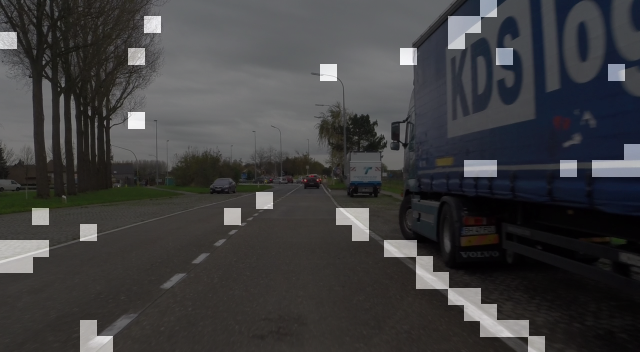
\includegraphics[width=\textwidth]{road1EXCLASSIFIER}
	\caption{Classificatie voor \texttt{road1.png}.}
\end{figure}
\begin{figure}
	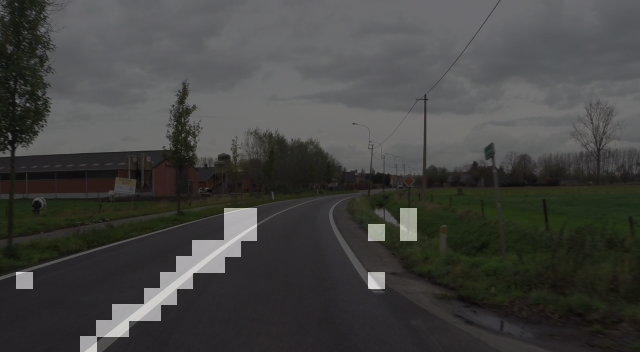
\includegraphics[width=\textwidth]{road2EXCLASSIFIER}
	\caption{Classificatie voor \texttt{road2.png}.}
\end{figure}
\begin{figure}
	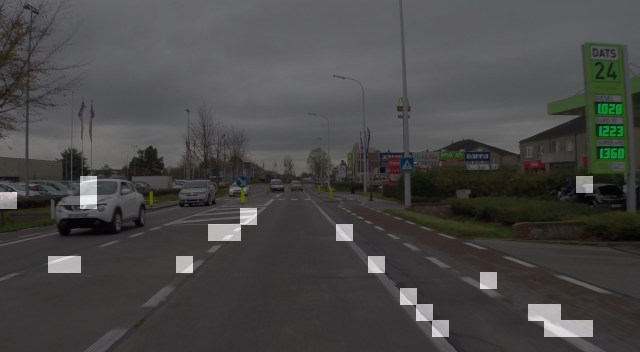
\includegraphics[width=\textwidth]{road3EXCLASSIFIER}
	\caption{Classificatie voor \texttt{road3.png}.}
\end{figure}
\begin{figure}
	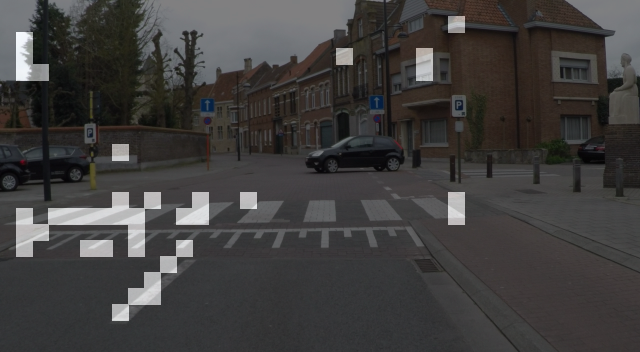
\includegraphics[width=\textwidth]{road4EXCLASSIFIER}
	\caption{Classificatie voor \texttt{road4.png}.}
\end{figure}


	
\end{document}